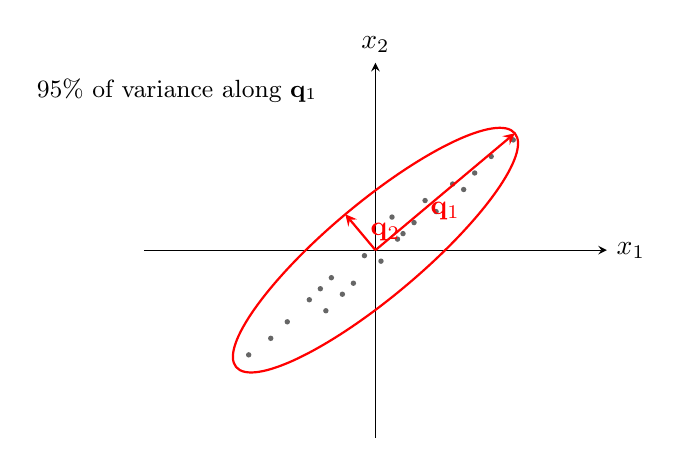
\begin{tikzpicture}[scale=0.7,>=stealth]
\draw[->] (-4.2,0)--(4.2,0) node[right]{$x_1$};
\draw[->] (0,-3.4)--(0,3.4) node[above]{$x_2$};
% scattered correlated data
\foreach \p in {(0.5,0.3),(-0.8,-0.5),(1.4,1.2),(-1.6,-1.3),(0.9,0.9),(-0.2,-0.1),(2.1,1.7),(-0.6,-0.8),(1.1,0.7),(-2.3,-1.9),(0.3,0.6),(-1.2,-0.9),(1.8,1.4),(-0.4,-0.6),(0.7,0.5),(-1.9,-1.6),(1.6,1.1),(0.1,-0.2),(-1.0,-0.7),(2.5,2.0),(0.4,0.2),(-0.9,-1.1)} \fill[black!60] \p circle (1.4pt);
\begin{scope}[rotate=40]
\draw[red,thick] (0,0) ellipse (3.3 and 0.85);
\draw[->,thick,red] (0,0)--(3.3,0) node[midway,below]{$\mathbf q_1$};
\draw[->,thick,red] (0,0)--(0,0.85) node[midway,right]{$\mathbf q_2$};
\end{scope}
\node at (-3.6,2.9) {\small 95\% of variance along $\mathbf q_1$};
\end{tikzpicture}
